\documentclass[11pt]{article}

%% MinionPro fonts 
%\usepackage[lf]{MinionPro}
%\usepackage{MnSymbol}
\usepackage{microtype}

%% Margins
\usepackage{geometry}
\geometry{verbose,letterpaper,tmargin=1in,bmargin=1in,lmargin=1in,rmargin=1in}

%% Other packages
\usepackage{amsmath}
\usepackage{amsthm}
\usepackage[shortlabels]{enumitem}
\usepackage{titlesec}
\usepackage{soul}
\usepackage{tikz}
\usepackage{mathtools}
\usepackage{pgfplots}
\usepackage{tikz-3dplot}
\usepackage{algorithmic}
\usepackage[export]{adjustbox}
\usepackage{tcolorbox}
\usepackage{mathrsfs}
\usepackage{hyperref}

%% Paragraph style settings
\setlength{\parskip}{\medskipamount}
\setlength{\parindent}{0pt}

%% Change itemize bullets
\renewcommand{\labelitemi}{$\bullet$}
\renewcommand{\labelitemii}{$\circ$}
\renewcommand{\labelitemiii}{$\diamond$}
\renewcommand{\labelitemiv}{$\cdot$}

%% Colors
\definecolor{rred}{RGB}{204,0,0}
\definecolor{ggreen}{RGB}{0,145,0}
\definecolor{yyellow}{RGB}{255,185,0}
\definecolor{bblue}{rgb}{0.2,0.2,0.7}
\definecolor{ggray}{RGB}{190,190,190}
\definecolor{ppurple}{RGB}{160,32,240}
\definecolor{oorange}{RGB}{255,165,0}

%% Shrink section fonts
\titleformat*{\section}{\normalsize\bf}
\titleformat*{\subsection}{\normalsize\bf}
\titleformat*{\subsubsection}{\normalsize\it}

% %% Compress the spacing around section titles
\titlespacing*{\section}{0pt}{1.5ex}{0.75ex}
\titlespacing*{\subsection}{0pt}{1ex}{0.5ex}
\titlespacing*{\subsubsection}{0pt}{1ex}{0.5ex}

%% amsthm settings
\theoremstyle{definition}
\newtheorem{problem}{Problem}
\newtheorem{example}{Example}
\newtheorem*{theorem}{Theorem}
\newtheorem*{bigthm}{Big Theorem}
\newtheorem*{biggerthm}{Bigger Theorem}
\newtheorem*{bigcor1}{Big Corollary 1}
\newtheorem*{bigcor2}{Big Corollary 2}

%% tikz settings
\usetikzlibrary{calc}
\usetikzlibrary{patterns}
\usetikzlibrary{decorations}
\usepgfplotslibrary{polar}

%% algorithmic setup
\algsetup{linenodelimiter=}
\renewcommand{\algorithmiccomment}[1]{\quad// #1}
\renewcommand{\algorithmicrequire}{\emph{Input:}}
\renewcommand{\algorithmicensure}{\emph{Output:}}

%% Answer box macros
%% \answerbox{alignment}{width}{height}
\newcommand{\answerbox}[3]{%
  \fbox{%
    \begin{minipage}[#1]{#2}
      \hfill\vspace{#3}
    \end{minipage}
  }
}

%% \answerboxfull{alignment}{height}
\newcommand{\answerboxfull}[2]{%
  \answerbox{#1}{6.38in}{#2} 
}

%% \answerboxone{alignment}{height} -- for first-level bullet
\newcommand{\answerboxone}[2]{%
  \answerbox{#1}{6.0in}{#2} 
}

%% \answerboxtwo{alignment}{height} -- for second-level bullet
\newcommand{\answerboxtwo}[2]{%
  \answerbox{#1}{5.8in}{#2}
}

%% special boxes
\newcommand{\wordbox}{\answerbox{c}{1.2in}{.7cm}}
\newcommand{\catbox}{\answerbox{c}{.5in}{.7cm}}
\newcommand{\letterbox}{\answerbox{c}{.7cm}{.7cm}}

%% Miscellaneous macros
\newcommand{\tstack}[1]{\begin{multlined}[t] #1 \end{multlined}}
\newcommand{\cstack}[1]{\begin{multlined}[c] #1 \end{multlined}}
\newcommand{\ccite}[1]{\only<presentation>{{\scriptsize\color{gray} #1}}\only<article>{{\small [#1]}}}
\newcommand{\grad}{\nabla}
\newcommand{\ra}{\ensuremath{\rightarrow}~}
\newcommand{\maximize}{\text{maximize}}
\newcommand{\minimize}{\text{minimize}}
\newcommand{\subjectto}{\text{subject to}}
\newcommand{\trans}{\mathsf{T}}
\newcommand{\bb}{\mathbf{b}}
\newcommand{\bx}{\mathbf{x}}
\newcommand{\bc}{\mathbf{c}}
\newcommand{\bd}{\mathbf{d}}

%% LP format
%    \begin{align*}
%      \maximize \quad & \mathbf{c}^{\trans} \mathbf{x}\\
%      \subjectto \quad & A \mathbf{x} = \mathbf{b}\\
%                       & \mathbf{x} \ge \mathbf{0}
%    \end{align*}


%% Redefine maketitle
\makeatletter
\renewcommand{\maketitle}{
  \noindent SA405 -- AMP \hfill Rader \S 3.4 \\

  \begin{center}\Large{\textbf{\@title}}\end{center}
}
\makeatother

%% ----- Begin document ----- %%
\begin{document}
  
\title{Lesson 11.  Traveling Sales(person) Problem (TSP)}

\maketitle

%%%
\section{Today...}

\begin{itemize}
	\item  Tours and TSP
	\item  Visiting Graduate Schools: IP (Integer-Programming) Formulation of TSP
\end{itemize}

\section{Tours and TSP}

\begin{tcolorbox}
A \textbf{tour} is a route that visits every location exactly once (and closes the ``loop'' by returning back where it started).

\smallskip
In graph terminology, a \textbf{tour} is a single \emph{cycle} that touches every node of the graph.
\end{tcolorbox}

\begin{problem}
For each graph below, does the set of edges represent a tour through the 6 nodes?  If not, explain why not.

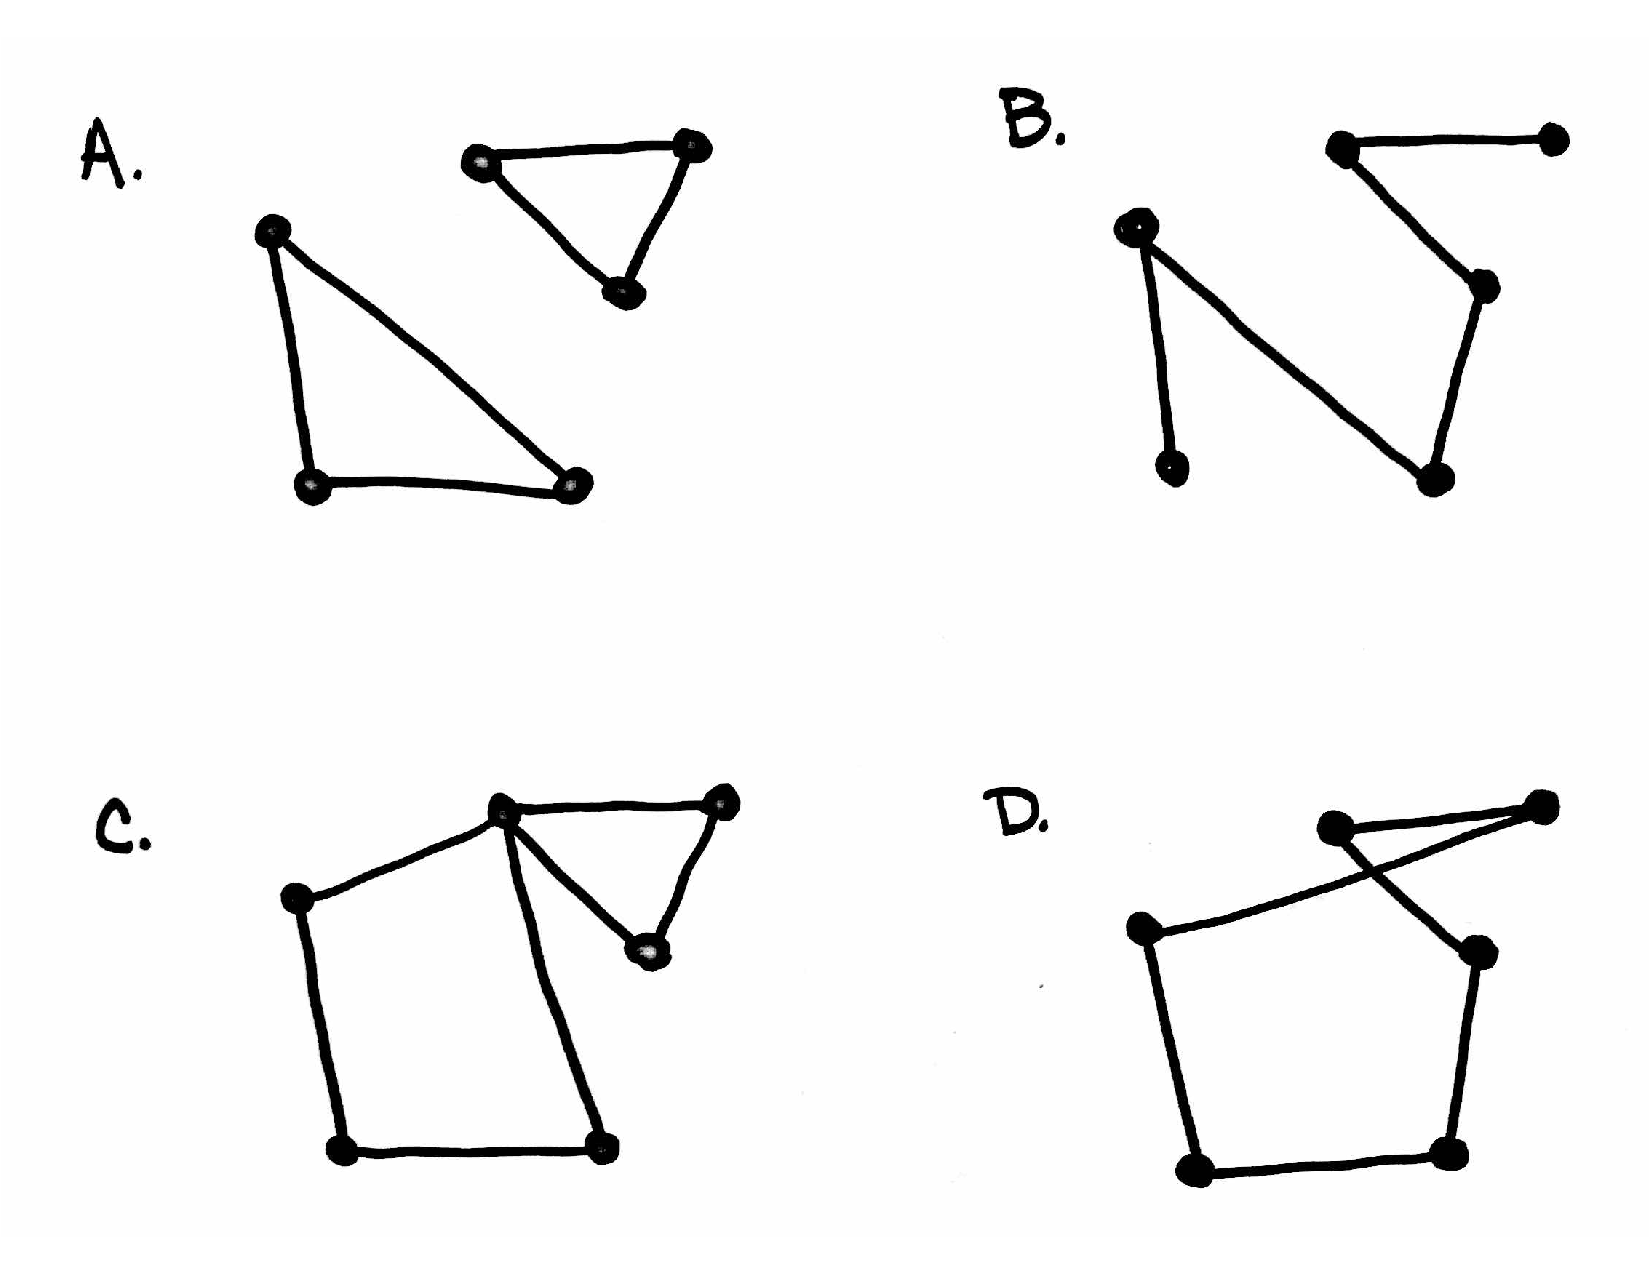
\includegraphics[width=0.7\textwidth]{tours}
\end{problem}

\begin{tcolorbox}
Given a graph $G = (V, E)$ with edge weights (representing costs or distances), the \textbf{Traveling Salesman Problem (TSP)} seeks a \emph{minimum cost tour of} $G$.
\end{tcolorbox}

\begin{problem}
TSP has a long and interesting history.  Look up TSP here \url{http://www.math.uwaterloo.ca/tsp}.  Write down a cool fact about TSP here.

\answerboxfull{c}{1.3cm}
\end{problem}


\section{Visiting Graduate Schools: IP Formulation of TSP}

\begin{problem}
A college student is interested in visiting as many graduate schools as possible.
She reasons that a single visit to each school is appropriate, and she wants to 
return to her own campus only after visiting all the schools.  It is conceivable that
she visits the schools in any order, but she would like to minimize the amount of
driving she has to do.  If the distance between schools $i$ and $j$ is $d_{i,j}$ ($i < j$), where the 
matrix $D$ of distances is given below, in which order should she visit the schools?
Note that school 1 is her current school.

\[
D = \left[
\begin{array}{c|ccccc}
& 2 & 3 & 4 & 5 & 6 \\
\hline
1 & 16 & 23 & 14 & 8 & 15 \\
2 & - & 12 & 19 & 9 & 13 \\
3 & - & - & 7 & 25 & 16 \\
4 & - & - & - & 18 & 15 \\
5 & - & - & - & - & 20 \\
\end{array}
\right]
\]

\begin{enumerate}[(a)]
\item Draw the graph $G = (V,E)$ of the network below.  Include node labels and edge costs.  Highlight a collection of edges that form a tour of the graph (doesn't have to be the minimum distance tour).

\answerboxone{c}{5cm}


\item Write a concrete model to minimize the cost of the edges used in a ``tour''.  Include constraints that ensure that each node touches exactly \catbox edges.  (Why?)

\answerboxone{c}{6.4cm}

\newpage
\item Do we have all of the constraints that we need?  Can you think of a collection of edges that satisfies the constraints we have so far, but that is not a tour? (Sketch it here.)

\answerboxone{c}{5cm}


\item Write a concrete constraint that prevents the graph that you sketched above from being selected by the solver.  

\answerboxone{c}{3cm}

\item Using parameterized notation, write a set of constraints that prevents ANY graphs of this kind from being returned by the solver.  There is such one constraint for every subset $C$ of vertices of $G$ such that \wordbox (restrict the number of vertices in $C$).  These are called \textbf{subtour elimination constraints}.

\answerboxone{c}{3cm}

\begin{tcolorbox}
For even a moderately sized problem, there are way too many \textbf{subtour elimination} constraints to add them ALL to the model.  In practice we could add these iteratively. Unlike the minimum spanning tree problem, we aren't guaranteed to have ``good'' success with this problem.  
\end{tcolorbox}

\end{enumerate}

\end{problem}

\end{document}

